% Copyright 2021 Joel Feldman, Andrew Rechnitzer and Elyse Yeager, except where noted.
% This work is licensed under a Creative Commons Attribution-NonCommercial-ShareAlike 4.0 International License.
% https://creativecommons.org/licenses/by-nc-sa/4.0/


%------------------------------------------------------
\section*{2.2 Definition of the Derivative}

 \begin{frame}{Table of Contents}
\mapofcontentsB{\bb}
 \end{frame}
 %--------
%----------------------------------------------------------------------------------------
\begin{frame}[t]{Derivative at a Point}
\begin{block}{Definition~\eref{text}{def:DIFFderiv}}
Given a function $f(x)$ and a point $a$, the slope of the tangent line to $f(x)$ at $a$ is the \alert{derivative of $f$ at $a$}, written \alert{$f'(a)$}.
\vspace{1cm}

So, $f'(a) = \displaystyle\lim_{h \rightarrow 0} \dfrac{f(a+h)-f(a)}{h}$.\
\vspace{1cm}

$f'(a)$ is also the \alert{instantaneous rate of change of $f$ at $a$}. 
\end{block}
\end{frame}
%----------------------------------------------------------------------------------------
\begin{frame}[t]
\begin{block}{Derivative}
\[f'(a) = \displaystyle\lim_{h \rightarrow 0} \dfrac{f(a+h)-f(a)}{h}\]
\end{block}

If $f'(a)>0$, then $f$ is \onslide<2->{\alert{increasing}} at $a$. \onslide<2->{Its graph ``points up."}

\pause\pause\vfill

If $f'(a)<0$, then $f$ is \onslide<4->{\alert{decreasing}} at $a$. \onslide<4->{Its graph ``points down."}

\vfill

\onslide<5->{If $f'(a)=0$, then $f$ looks \alert{constant} or \alert{flat} at $a$.}

\StatusBar{1}{5}
\end{frame}
%-----------------------------------------------
%------------------------------------------------------------------
\begin{frame}[t]{Practice: Increasing and Decreasing}

\begin{center}
\begin{tikzpicture}
\myaxis{x}{0}{4.5}{y}{0}{4}

\begin{scope}
\clip (0,0) rectangle (4.2,4.2); \draw[C2, ultra thick] (0,0) .. controls (1,5) and (3,-2) .. (4.5,4.5);
\end{scope}

\onslide<2->{
\draw[dashed] (.8,0)--(.8,1.85) node[vertex]{};
\draw (.8,0) node[below, M4]{$a$};
}

\onslide<2->{
\draw[dashed] (2,0)--(2,1.7) node[vertex]{};
\draw (2,0) node[below, C4]{$b$};
}

\onslide<2->{
\draw[dashed] (2.75,0)--(2.75,1.525) node[vertex]{};
\draw (2.75,0) node[below, green]{$c$};
}

\onslide<2->{
\draw[dashed] (4,0)--(4,2.9) node[vertex]{};
\draw (4,0) node[below, M5]{$d$};
}
\end{tikzpicture}
\end{center}

\only<3,4>{Where is $f'(x)<0$?\quad}  \answer{\only<4>{{\color{C4}$f'(b)<0$}}}
\only<5,6>{Where is $f'(x)>0$?\quad} \answer{\only<6>{{\color{M4}$f'(a)>0$} and {\color{M5}$f'(d)>0$}}}
\only<7,8>{Where is $f'(x)\approx0$?\quad} \answer{\only<8>{{\color{M3}$f'(c)\approx 0$}}}
\vfill

\only<3,5,7>{\AnswerYes}
\only<3>{\QuestionBar{1}{3}}
\only<4>{\AnswerBar{1}{3}}
\only<5>{\QuestionBar{2}{3}}
\only<6>{\AnswerBar{2}{3}}
\only<7>{\QuestionBar{3}{3}}
\only<8>{\AnswerBar{3}{3}}
\end{frame}

%----------------------------------------------------------------------------------------
\begin{frame}[t]
Use the definition of the derivative to find the slope of the tangent line to $f(x)=x^2-5$ at the point $x=3$.

\answer{\parbox{.25\textwidth}{
\begin{tikzpicture}[yscale=0.5]
\begin{scope}[xshift=1cm]\myaxis{\only<1-3>{x}}{0}{4}{y}{0.5}{6}\end{scope}
\draw[C2, ultra thick, domain=2:4.1] plot (\x, {.5*\x*\x-2.5});
\draw[dashed] (3,2)--(3,-.2) node[below]{3};
\onslide<2->{\draw[dashed] (4,5.5)--(4,-.2)node[below,xshift=3mm]{$3+h$};}
\onslide<3->{\draw[dashed] (1,5.5)-- (4,5.5) node[vertex]{};
\draw[dashed] (1,2)-- (3,2) node[vertex]{};
\draw (1,5.5) node[right,fill=white,inner sep=0]{$f(3+h)$};
\draw (1,2) node[right,fill=white,inner sep=0]{$f(3)$};}
\end{tikzpicture}}
\hfill\color{answercolor}
\onslide<4>{\parbox{.25\textwidth}{\small
\begin{align*}
f'(3)&=\lim_{h \rightarrow 0}\dfrac{\textcolor{M4}{f(3+h)}-\textcolor{C4}{f(3)}}{h}\\
&=\lim_{h \rightarrow 0}\dfrac{\textcolor{M4}{\left((3+h)^2-5\right)}-\textcolor{C4}{(3^2-5)}}{h}\\
&=\lim_{h \rightarrow 0}\dfrac{\textcolor{M4}{\left(9+6h+h^2-5\right)}-\textcolor{C4}{4}}{h}\\
&=\lim_{h \rightarrow 0}\dfrac{h^2+6h}{h}\\
&=\lim_{h \rightarrow 0}{h+6}=6
\end{align*}}}
}
\only<1-3>{\AnswerYes}
\unote{Example~\eref{text}{eg:DIFFderivX2}}
\end{frame}
%------------------------------------------------------------------
%------------------------------------------------------------------
%----------------------------------------------------------------------------------------
\begin{frame}[t]
Let's keep the function $f(x)=x^2-5$. We just showed $f'(3)=6$.
\qquad
We can also find its derivative at an arbitrary point $x$:\color{answercolor}
\pause

\answer{\begin{align*}
f'(x) &= \lim_{h \rightarrow 0}\dfrac{\textcolor{M4}{f(x+h)}-\textcolor{C4}{f(x)}}{h}\\
& = \lim_{h \rightarrow 0}\dfrac{\textcolor{M4}{(x+h)^2-5}-\textcolor{C4}{(x^2-5)}}{h}\\
&=\lim_{h \rightarrow 0}\frac{\textcolor{M4}{x^2+2xh+h^2-5}-\textcolor{C4}{x^2+5}}{h}\\
&=\lim_{h \rightarrow 0}\frac{2xh+h^2}{h}\\
&=\lim_{h \rightarrow 0}{2x+h}=\alert{2x}  \qquad \mbox{(In particular, $f'(3)=6$.)}
\end{align*}}
\only<1>{\AnswerYes}
\end{frame}
%------------------------------------------------------------------
%----------------------------------------------------------------------------------------
\begin{frame}[t]
\begin{center}
\begin{tikzpicture}[yscale=0.75]
\myaxis{x}{3}{3}{y}{5.5}{4.5}
\draw[ultra thick, C2, domain=-3:3] plot[samples=100] (\x,{\x*\x-5}) node[right]{$f(x)=x^2-5$};
\draw[ultra thick, M4, domain=-2.5:2.5] plot (\x,{2*\x}) node[right]{$f'(x)=2x$};
\end{tikzpicture}
\end{center}
\end{frame}
%------------------------------------------------------------------
%-------------------------------------------------------------------
\begin{frame}{Increasing and Decreasing}
In black is the curve $y=f(x)$. Which of the coloured curves corresponds to $y=f'(x)$?
\begin{center}
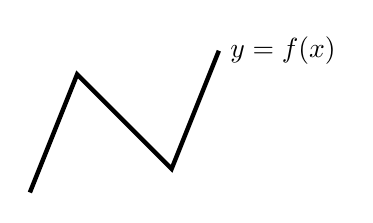
\begin{tikzpicture}[scale=0.3]
\myaxis{x}{4}{4}{y}{3}{3}
\draw[ultra thick] (-4,-3)--(-2,2)--(2,-2)--(4,3) node[right]{$y=f(x)$};
\end{tikzpicture}

\begin{tikzpicture}[scale=0.3]
\myaxis{x}{4}{4}{y}{3}{3}
\draw[very thick, M4] (-4,.83)--(-2,.83) (-2,-1)--(2,-1) (2,.83)--(4,.83);
\draw[M4] (0,-4) node{$A$};
\end{tikzpicture}\hfill
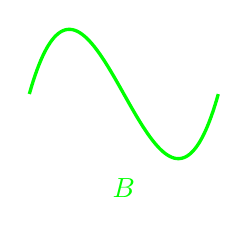
\begin{tikzpicture}[scale=0.3]
\myaxis{x}{4}{4}{y}{3}{3}
\draw[very thick, green] plot[domain=-4:4, samples=100](\x,{\x*(\x-4)*(\x+4)/9});
\draw[green] (0,-4) node{$B$};
\end{tikzpicture}\hfill
\begin{tikzpicture}[scale=0.3]
\myaxis{x}{4}{4}{y}{3}{3}
\draw[very thick, C4] (-4,3)--(-2,-2)--(2,2)--(4,-3);
\draw[C4] (0,-4) node{$C$};
\end{tikzpicture}
\end{center}

\QuestionBar{1}{2}\AnswerNo
\end{frame}
%--------------------------------------------------------------------

\begin{frame}{Increasing and Decreasing}
In black is the curve $y=f(x)$. Which of the coloured curves corresponds to $y=f'(x)$?
\begin{center}
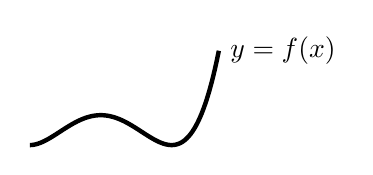
\begin{tikzpicture}[scale=0.3]
\myaxis{x}{4}{4}{y}{3}{3}
\draw[ultra thick] plot[domain=-4:4, samples=100](\x,{(\x+4)*(\x+4)*(\x-2)*(\x-2)/64}) node[right]{$y=f(x)$};
\end{tikzpicture}

\begin{tikzpicture}[scale=0.3]
\myaxis{x}{4}{4}{y}{3}{3}
\draw[very thick, M4] plot[domain=-4:4, samples=100](\x,{(\x-2)*(\x+4)*(\x+4)/32});
\draw[M4] (0,-4) node{$A$};
\end{tikzpicture}\hfill
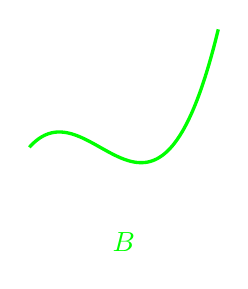
\begin{tikzpicture}[scale=0.3]
\myaxis{x}{4}{4}{y}{3}{3}
\draw[very thick, green] plot[domain=-4:4, samples=100](\x,{(\x+4)*(\x-2)*(\x+1)/16});
\draw[green] (0,-4) node{$B$};
\end{tikzpicture}\hfill
\begin{tikzpicture}[scale=0.3]
\myaxis{x}{4}{4}{y}{3}{3}
\draw[very thick, C4] plot[domain=-4:4, samples=100](\x,{\x+.5*sin(1.5*\x r)});
\draw[C4] (0,-4) node{$C$};
\end{tikzpicture}
\end{center}
\QuestionBar{2}{2}\AnswerNo
\end{frame}
%-------------------------------------------------------------------
%----------------------------------------------------------------------------------------
\begin{frame}[t]
\begin{block}{Derivative as a Function -- Definition~\eref{text}{def:DIFFderivFunc}}
Let $f(x)$ be a function.

The derivative of $f(x)$ with respect to $x$ is given by
\[f'(x)=\lim_{h \rightarrow 0}\frac{f(x+h)-f(x)}{h},\]
provided the limit exists. Notice that $x$ will be a part of your final expression: this is a \alert{function}.\\$ $\\

If $f'(x)$ exists for all $x$ in an interval $(a,b)$, we say that $f$ is \alert{differentiable on $(a,b)$}.
\end{block}
\end{frame}
%----------------------------------------------------------------------------------------
\begin{frame}
\begin{block}{Notation \eref{text}{notn higher diff}}
The ``prime" notation $f'(x)$ and $f'(a)$ is sometimes called Newtonian notation. We will also use Leibnitz notation:
\begin{align*}
\diff{f}{x}&& \diff{f}{x}(a) && \diff{}{x}f(x) && \left.\diff{}{x}f(x)\right|_{x=a}\\
\onslide<2->{
\color{M3}\text{function} && \color{M5}\text{number} && \color{M3}\text{function} && \color{M5}\text{number}
}\end{align*}
\end{block}
\end{frame}
%----------------------------------------------------------------------------------------
\begin{frame}[t]
Newtonian Notation:
\[f(x)=x^2+5 \hspace{1cm} f'(x)=2x \hspace{1cm} f'(3)=6\]
\vfill

Leibnitz Notation:\\[1em]
$\ds\diff{f}{x}=\answer{\onslide<2->{\textcolor{answercolor}{2x}}}$ \hfill $\ds\diff{f}{x}(3)=\answer{\onslide<3->{\textcolor{answercolor}{6}}}$ \hfill $\ds\diff{}{x}f(x)=\answer{\onslide<4->{\textcolor{answercolor}{2x}}}$ \hfill $\left.\ds\diff{}{x}f(x)\right\vert_{x=3}=\answer{\onslide<5->{\textcolor{answercolor}6}}$

\vfill
\begin{center}
\begin{tikzpicture}[yscale=0.3]
\myaxis{x}{3}{3}{y}{5.5}{4.5}
\draw[ultra thick, C2, domain=-3:2.6] plot (\x,{\x*\x-5}) node[right]{$f(x)=x^2-5$};
\draw[ultra thick, M4, domain=-2.5:2.5] plot (\x,{2*\x}) node[right]{$f'(x)=2x$};
\end{tikzpicture}
\end{center}

\only<-4>{\AnswerYes}
\end{frame}
%----------------------------------------------------------------------------------------
\begin{frame}[t]
\begin{block}{Alternate Definition -- Definition \eref{text}{def:DIFFderiv}}
Calculating
\[f'(a)=\lim_{h \rightarrow 0}\frac{f(a+h)-f(a)}{h}\]
is the same as calculating
\[f'(x)=\lim_{x \rightarrow a}\frac{f(x)-f(a)}{x-a}.\]
Notice in these scenarios, $h=x-a$.
\end{block}
\begin{center}
\begin{tikzpicture}
\draw[thick] (0,0)--(5,0);
\draw (1,.25)--(1,-.25) node[below, C2]{$a$};
\draw (1,0) node[vertex]{};
\draw (3,.25)--(3,-.25) node[below]{$x$};
\draw (3,0) node[vertex]{};
\draw[<->] (1,.35)--(3,.35); 
\draw (2,.5) node{$h$} ;
\end{tikzpicture}
\end{center}
\end{frame}
%----------------------------------------------------------------------------------------
\begin{frame}[t]%{Using the Definition of a Derivative}
Let $f(x)=\sqrt{x}$. Using the definition of a derivative, calculate $f'(x)$.\pause

\answer{\color{answercolor}
\begin{align*}
f'(x) &= \lim_{h \rightarrow 0}\dfrac{f(x+h)-f(x)}{h}\\
&= \lim_{h \rightarrow 0}\dfrac{\sqrt{x+h}-\sqrt{x}}{h}\\
&= \lim_{h \rightarrow 0}\dfrac{\sqrt{x+h}-\sqrt{x}}{h}\left(\dfrac{\sqrt{x+h}+\sqrt{x}}{\sqrt{x+h}+\sqrt{x}}\right)\\
&= \lim_{h \rightarrow 0}\dfrac{(x+h)-(x)}{h(\sqrt{x+h}+\sqrt{x})}\\
&= \lim_{h \rightarrow 0}\dfrac{1}{\sqrt{x+h}+\sqrt{x}}=\dfrac{1}{2\sqrt{x}}
\end{align*}}
\unote{Example~\eref{text}{eg:DIFFderivXsqrt}}
\end{frame}
%----------------------------------------------------------------------------------------
\begin{frame}
\only<2>{\AnswerYes \QuestionBar{2}{4}}
\only<3>{\AnswerBar{1}{4}}
\only<4>{\AnswerBar{2}{4}}
\only<5>{\AnswerYes \QuestionBar{4}{4}}
\only<6>{\AnswerBar{3}{4}}
\only<7>{\AnswerBar{4}{4}}

\begin{tikzpicture}
\myaxis{x}{0}{10.5}{y}{1}{4}
\draw[C2, ultra thick, domain=0:10] plot[ samples=200] (\x, {sqrt(\x)}) node[below]{$y=\sqrt{x}$};
\draw[M4, ultra thick, domain=.03:10] plot[ samples=200] (\x, {.5/sqrt(\x)}) node[above]{$y=\frac{1}{2\sqrt{x}}$};\end{tikzpicture}\pause
\vfill

\fbox{Review:}\hspace{1cm}
$\dlimx{\infty}\sqrt{x}=\answer{\onslide<3->{\textcolor{answercolor}\infty}}$ \hspace{1cm}
$\dlimx{\infty}\dfrac{1}{2\sqrt{x}} = \answer{\onslide<4->{\textcolor{answercolor}0}}$\\
\onslide<5->{$\dlimx{0^+}\sqrt{x}=\answer{\onslide<6->{\textcolor{answercolor}0}}$ \hspace{1cm}
$\dlimx{0^+}\dfrac{1}{2\sqrt{x}} =\answer{ \onslide<7->{\textcolor{answercolor}\infty}}$}
\vfill
\end{frame}
%----------------------------------------------------------------------------------------
\begin{frame}[t]
\only<1>{\AnswerYes \QuestionBar{1}{3}}
\only<2->{\AnswerBar{1}{3}}
\NowYou ~ Using the definition of the derivative, calculate $\ds\diff{}{x}\left\{\dfrac{1}{x}\right\}$.\pause\color{answercolor}
\answer{\begin{align*}
\diff{}{x}\left[\frac{1}{x}\right]&=\lim_{h \rightarrow 0} \dfrac{\frac{1}{x+h}-\frac{1}{x}}{h}\\
&=\lim_{h \rightarrow 0}\frac{\frac{x}{x(x+h)}-\frac{x+h}{x(x+h)}}{h}\\
&=\lim_{h \rightarrow 0}\frac{\frac{-h}{x(x+h)}}{h}\\
&=\lim_{h \rightarrow 0}\frac{-1}{x(x+h)}
=-\frac{1}{x^2}
\end{align*}}
\color{black}
\unote{Example~\eref{text}{eg:DIFFderivXm1}}
\end{frame}
%----------------------------------------------------------------------------------------
\answer{\begin{frame}
\QuestionBar{3}{3}
\AnswerYes \MoreSpace
\note<1>{Two questions are on the same slide so students can see both at the same time. Faster workers can finish the first and move on to the second, while slower workers have time to really make progress on the first. ``Focus hard on getting as far as you can with the first question. If you're super speedy and finish it before your classmates, you can start to work on the second."}


\NowYou ~ Using the definition of the derivative, calculate $\ds\diff{}{x}\left\{\dfrac{2x}{x+1}\right\}$.
\vfill

\NowYou ~ Using the definition of the derivative, calculate $\ds\diff{}{x}\left\{\dfrac{1}{\sqrt{x^2+x}}\right\}$.
\vfill
\end{frame}}
%----------------------------------------------------------------------------------------
\begin{frame}[t]
\only<1>{\QuestionBar{2}{3}\AnswerYes}
\only<2>{\AnswerBar{2}{3}}
Using the definition of the derivative, calculate $\ds\diff{}{x}\left\{\dfrac{2x}{x+1}\right\}$.
\color{answercolor}\pause

\small
\answer{\begin{align*}\lim_{h \rightarrow 0}&\frac{f(x+h)-f(x)}{h}=\lim_{h \rightarrow 0}\frac{\frac{2(x+h)}{x+h+1}-\frac{2x}{x+1}}{h}\\
&=\lim_{h \to 0}\frac{1}{h}\left(\tfrac{2(x+h)(x+1)}{(x+h+1)(x+1)}-\tfrac{2x(x+h+1)}{(x+1)(x+h+1)}\right)\\
&=\lim_{h \to 0}\frac{2}{h}\left(\frac{(x^2+x+xh+h)-(x^2+xh+x)}{(x+h+1)(x+1)}\right)\\
&=\lim_{h \to 0}\frac{2}{h}\left(\frac{h}{(x+h+1)(x+1)}\right)\\
&=\lim_{h \to 0}\frac{2}{(x+h+1)(x+1)}=\frac{2}{(x+1)^2}
\end{align*}}
\end{frame}
%----------------------------------------------------------------------------------------
\begin{frame}[t]
\only<1>{\QuestionBar{3}{3}\AnswerYes}
\only<2>{\AnswerBar{3}{3}}

Using the definition of the derivative, calculate $\ds\diff{}{x}\left\{\dfrac{1}{\sqrt{x^2+x}}\right\}$.
\pause

\color{answercolor}\footnotesize
\answer{\begin{align*}
&\lim_{h \to 0}\frac{f(x+h)-f(x)}{h}=\lim_{h \to 0} \frac{\frac{1}{\sqrt{(x+h)^2+x+h}}-\frac{1}{\sqrt{x^2+x}}}{h}\\
&=\lim_{h \to 0}\frac{1}{h}\left(
\tfrac{\sqrt{x^2+x}}{\sqrt{(x^2+h)^2+x+h}\sqrt{x^2+x}}-\tfrac{\sqrt{(x+h)^2+x+h}}{\sqrt{(x^2+h)^2+x+h}\sqrt{x^2+x}}
\right)\\
&=\lim_{h \to 0}\frac{1}{h}\left(
\tfrac{\sqrt{x^2+x}-\sqrt{(x+h)^2+x+h}}{\sqrt{(x^2+h)^2+x+h}\sqrt{x^2+x}}
\right)\left(\tfrac{\sqrt{x^2+x}+\sqrt{(x+h)^2+x+h}}{\sqrt{x^2+x}+\sqrt{(x+h)^2+x+h}}\right)\\
&=\lim_{h \to 0}\frac{1}{h}\left(
\tfrac{(x^2+x)-[(x+h)^2+x+h]}{\sqrt{(x^2+h)^2+x+h}\sqrt{x^2+x}\left[\sqrt{x^2+x}+\sqrt{(x+h)^2+x+h}\right]}
\right)\\
&=\lim_{h \to 0}\frac{1}{h}\left(
\tfrac{-(2xh+h^2+h)}{\sqrt{(x^2+h)^2+x+h}\sqrt{x^2+x}\left[\sqrt{x^2+x}+\sqrt{(x+h)^2+x+h}\right]}
\right)\\
&=\lim_{h \to 0}
\tfrac{-(2x+h+1)}{\sqrt{(x^2+h)^2+x+h}\sqrt{x^2+x}\left[\sqrt{x^2+x}+\sqrt{(x+h)^2+x+h}\right]}=\tfrac{-(2x+1)}{2(x^2+x)^{3/2}}
\end{align*}}

\end{frame}
%----------------------------------------------------------------------------------------

%----------------------------------------------------------------------------------------
\begin{frame}
\begin{block}{Memorize}
The derivative of a function $f$ at a point $a$ is given by the following limit, if it exists:
\[f'(a) = \lim_{h\rightarrow 0} \frac{f(a+h)-f(a)}{h}\]
\end{block}
\end{frame}
%----------------------------------------------------------------------------------------



%----------------------------------------------------------------------------------
\begin{frame}{Zooming In}
For a smooth function, if we zoom in at a point, we see a line:
\begin{center}
\hfill\begin{tikzpicture}
\myaxis{}{.5}{2}{}{.5}{2}
\draw[thick, C1] plot[domain=-.5:2, samples=50, smooth](\x,{1-\x*\x+\x*\x*\x/2});
\draw[M4] (1,.5) node[vertex]{};
\xcoord{1}{1}
\xcoord{2}{2}
\ycoord{1}{1}
\ycoord{2}{2}
\draw[dotted, gray] (-.5,-.5) grid[step=0.5] (2,2);
\onslide<2->{\draw[M3] (1,.5) node[shape=rectangle, minimum size=1cm, draw]{};}
\end{tikzpicture}
\hfill
\onslide<3->{\begin{tikzpicture}
\draw[thick, C1] plot[domain=.5:1.5, samples=50, smooth, scale=2](\x,{1-\x*\x+\x*\x*\x/2});
\draw[dotted, gray] (1,0) grid[step=0.5] (3,2);
\draw[M3] (2,1) node[shape=rectangle, minimum size=2cm, draw]{};
\onslide<4->{\draw[M5] (2,1) node[shape=rectangle, minimum size=1cm, draw]{};}
\draw[M4] (2,1) node[vertex]{};
\xcoord{2}{1}
\xcoord{3}{1.5}
\end{tikzpicture}}\hfill
\onslide<5->{\begin{tikzpicture}
\draw[thick, C1] plot[domain=.75:1.25, samples=50, smooth, scale=4](\x,{1-\x*\x+\x*\x*\x/2});
\draw[dotted, gray] (3,1) grid[step=0.5] (5,3);
\draw[M5] (4,2) node[shape=rectangle, minimum size=2cm, draw]{};
\begin{scope}[yshift=1cm]
\xcoord{4}{1}
\xcoord{5}{1.25}
\end{scope}
\onslide<6->{\draw[M4] (4,2) node[shape=rectangle, minimum size=1cm, draw]{};}
\draw[M4] (4,2) node[vertex]{};
\end{tikzpicture}}\hfill
\onslide<7->{\begin{tikzpicture}
\draw[thick, C1] plot[domain=.875:1.125, samples=50, smooth, scale=8](\x,{1-\x*\x+\x*\x*\x/2});
\draw[dotted, gray] (7,3) grid[step=0.5] (9,5);
\draw[M4] (8,4) node[vertex]{};
\draw[M4] (8,4) node[shape=rectangle, minimum size=2cm, draw]{};
\begin{scope}[yshift=3cm]
\xcoord{8}{1}
\xcoord{9}{1.25}
\end{scope}
\end{tikzpicture}}
\hfill~
\end{center}
\vfill
\onslide<8->{In this example, the slope of our zoomed-in line looks to be about:
\[\frac{\Delta y}{\Delta x}  \approx -\frac{1}{2}\]}
\vfill
\StatusBar{1}{7}
\end{frame}

%----------------------------------------------------------------------------------------

%--------------------------------------
\begin{frame}{Zooming in on  functions that aren't smooth}
For a function with a cusp or a discontinuity, even though we zoom in very closely, we don't see simply a single straight line.

\begin{center}
\hfill\begin{tikzpicture}
\draw (-.75,1) node[left]{Cusp:};
\myaxis{}{.5}{2}{}{.5}{2}
\draw[thick, C1] plot[domain=-.5:1, samples=50, smooth](\x,{.75+sqrt(1-\x)});
\draw[thick, C1] plot[domain=1:2, samples=50, smooth](\x,{.75+sqrt(\x-1)});
\xcoord{1}{1}
\xcoord{2}{2}
\draw[dotted, gray] (-.5,-.5) grid[step=0.5] (2,2);
\onslide<2->{\draw[M3] (1,1) node[shape=rectangle, minimum size=1cm, draw]{};}
\end{tikzpicture}
\hfill
\onslide<3->{\begin{tikzpicture}
\draw[thick, C1] plot[domain=0.5:1, samples=50, smooth](\x*2,{1.5+2*sqrt(1-\x)});
\draw[thick, C1] plot[domain=1:1.5, samples=50, smooth](\x*2,{1.5+2*sqrt(\x-1)});
\draw[dotted, gray] (1,1) grid[step=0.5] (3,3);
\draw[M3] (2,2) node[shape=rectangle, minimum size=2cm, draw]{};
\onslide<4->{\draw[M5] (2,1.75) node[shape=rectangle, minimum size=1cm, draw]{};}
\begin{scope}[yshift=1cm]
\xcoord{2}{1}
\xcoord{3}{1.5}
\end{scope}
\end{tikzpicture}}\hfill
\onslide<5->{\begin{tikzpicture}
\draw[thick, C1] plot[domain=0.875:1, samples=50, smooth](\x*4,{3+4*sqrt(1-\x)});
\draw[thick, C1] plot[domain=1:1.125, samples=50, smooth](\x*4,{3+4*sqrt(\x-1)});
\draw[dotted, gray] (3,2.5) grid[step=0.5] (5,4.5);
\draw[M5] (4,3.5) node[shape=rectangle, minimum size=2cm, draw]{};
\begin{scope}[yshift=2.5cm]
\xcoord{4}{1}
\xcoord{5}{1.25}
\end{scope}
\end{tikzpicture}}
\hfill~
\end{center}

\onslide<6->{
\begin{center}
\hfill\begin{tikzpicture}
\draw (-.75,1) node[left]{Discontinuity:};
\myaxis{}{.5}{2}{}{.5}{2}
\draw[thick, C1] plot[domain=-.5:1, samples=50, smooth](\x,{.5+sin(\x*1.6 r)});
\draw[thick, C1] plot[domain=1:2, samples=50, smooth](\x,{.25+sin(\x*1.6 r)});
\xcoord{1}{1}
\xcoord{2}{2}
\draw[dotted, gray] (-.5,-.5) grid[step=0.5] (2,2);
\onslide<7->{\draw[M3] (1,1.25) node[shape=rectangle, minimum size=1cm, draw]{};}
\end{tikzpicture}
\hfill
\onslide<8->{\begin{tikzpicture}
\draw[thick, C1] plot[domain=.5:1, samples=50, smooth, scale=2](\x,{.5+sin(\x*1.6 r)});
\draw[thick, C1] plot[domain=1:1.5, samples=50, smooth, scale=2](\x,{.25+sin(\x*1.6 r)});
\draw[M3] (2,2.5) node[shape=rectangle, minimum size=2cm, draw]{};
\draw[dotted, gray] (1,1.5) grid[step=0.5] (3,3.5);
\onslide<9->{\draw[M5] (2,2.75) node[shape=rectangle, minimum size=1cm, draw]{};}
\begin{scope}[yshift=1.5cm]
\xcoord{2}{1}
\xcoord{3}{1.5}
\end{scope}
\end{tikzpicture}}\hfill
\smash{\onslide<10->{\begin{tikzpicture}
\iftoggle{printsolutions}{
\onslide<11>{
\index{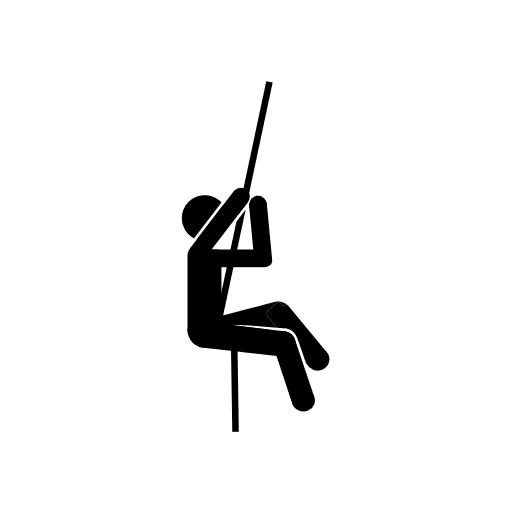
\includegraphics[height=10mm]{Clipart/climb.png} 
\href{https://thenounproject.com/icon/16371/}{'Rope Climbing} by \href{https://thenounproject.com/AVAROP/}{\'Alvaro Papilla Marraqueta } is licensed under
\CCBYthree~ (accessed 13 September 2018)}
\draw (3.9,5.5) node[rotate=-15,xscale=-1]{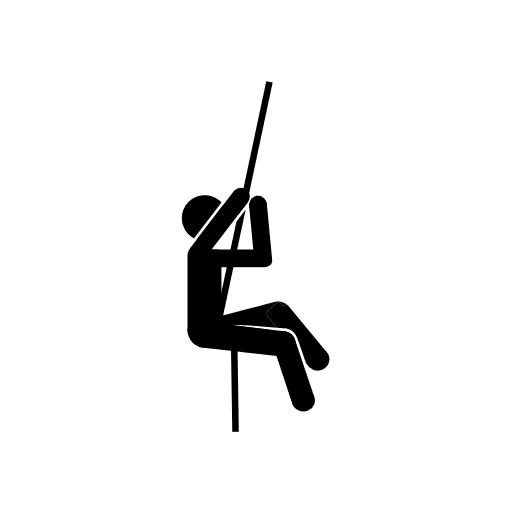
\includegraphics[height=15mm]{Clipart/climb.png}};}}{}
\draw[thick, C1] plot[domain=.75:1, samples=50,smooth, scale=4](\x,{.5+sin(\x*1.6 r)});
\draw[thick, C1] plot[domain=1:1.25, samples=50,smooth, scale=4](\x,{.25+sin(\x*1.6 r)});
\draw[M5] (4,5.5) node[shape=rectangle, minimum size=2cm, draw]{};
\draw[dotted, gray] (3,4.5) grid[step=0.5] (5,6.5);
\begin{scope}[yshift=4.5cm]
\xcoord{4}{1}
\xcoord{5}{1.25}
\end{scope}
\end{tikzpicture}}}\hfill~
\end{center}}
\end{frame}

%----------------------------------------------------------------------------------------
%----------------------------------------------------------------------------------
\begin{frame}
\begin{block}{Alternate Definition -- Definition \eref{text}{def:DIFFderiv}}
Calculating
\[f'(a)=\lim_{h \rightarrow 0}\frac{f(a+h)-f(a)}{h}\]
is the same as calculating
\[f'(x)=\lim_{x \rightarrow a}\frac{f(x)-f(a)}{x-a}.\]
Notice in these scenarios, $h=x-a$.
\end{block}


The derivative of $f(x)$ \alert{does not exist} at $x=a$ if
\[\lim_{x \to a}\frac{f(x)-f(a)}{x-a}\]
does not exist.\\ Note this is the slope of the tangent line to $y=f(x)$ at $x=a$, $\frac{\Delta y}{\Delta x}$.
\end{frame}
%----------------------------------------------------------------------------------
\begin{frame}[t]{When Derivatives Don't Exist}
\unote{Example~\eref{text}{eg:DIFFderivXthird}}
What happens if we try to calculate a derivative where none exists?\\[1em]

\textcolor{C1}{Find the derivative of $f(x) =x^{1/3} $ at $x=0$.}
\onslide<2-|handout:0>{\color{answercolor}
\begin{multicols}{2}
\begin{align*}
f'(0)&=\lim_{h \to 0}\frac{f(h)-f(0)}{h}\\
&=\lim_{h \to 0} \frac{h^{1/3}-0}{h}\\
&=\lim_{h \to 0}\frac{1}{h^{2/3}}=\infty
\end{align*}
Since the limit does not exist, we conclude $f'(x)$ is not defined at $x=0$.\columnbreak

We can go a little farther: since the limit goes to infinity, the graph $y=f(x)$ looks vertical at $x=0$.

\begin{tikzpicture}
\myaxis{x}{2}{2}{y}{1}{1}
\draw[thick,C1] plot[domain=-1:1,xscale=2]({\x*\x*\x},{\x});
\end{tikzpicture}
\end{multicols}}
\note<2>{As usual, it's nice to reassure students that we did not need to know the graph of this function to answer the question. Otherwise, they might unduly worry.}
\end{frame}

%----------------------------------------------------------------------------------------

%----------------------------------------------------------------------------------
\begin{frame}[t]
\only<1>{\AnswerYes}
\begin{block}{Theorem~\eref{text}{thm:DIFFdiffGivesCont}}
If the function $f(x)$ is differentiable at $x=a$, then $f(x)$ is also continuous at $x=a$.
\end{block}
Proof:\qquad
\onslide<2|handout:0>{\color{answercolor}
If $f'(a)$ exists, that means:
\begin{align*}
\lim_{h \to 0}\frac{f(a+h)-f(a)}{h} &\qquad \mbox{exists}\\
\implies \lim_{h \to 0}\left[\alert{h}\cdot \frac{f(a+h)-f(a)}{h} \right]&=\left[\lim_{h \to 0}\alert{h}\right]\cdot \left[\lim_{h \to 0}\frac{f(a+h)-f(a)}{h}\right] \\
\implies \lim_{h \to 0}\left[\alert{h}\cdot \frac{f(a+h)-f(a)}{h} \right]&=0\\
\implies \lim_{h \to 0}\left[f(a+h)-f(a) \right]&=0
\\\implies \lim_{h \to 0} f(a+h)&= f(a)
\end{align*}
and that is the definition of $f(x)$ being continuous at $x=a$.
}
\end{frame}

%----------------------------------------------------------------------------------------
\begin{frame}[t]%{Concept Check}
Let $f(x)$ be a function and let $a$ be a constant in its domain. Draw a picture of each scenario, or say that it is impossible.

\iftoggle{printsolutions}{
\begin{tabular}{|c|c|}
\hline
\parbox{.45\textwidth}{$f(x)$ continuous at $x=a$\\
$f(x)$ differentiable at $x=a$\\
\onslide<2>{\begin{center}\begin{tikzpicture}
\xcoord{0}{a}
\draw[C1,thick] plot[domain=-1:1](\x,{\x/2});
\end{tikzpicture}\end{center}}}
&
\parbox{.45\textwidth}{$f(x)$ continuous at $x=a$\\
$f(x)$ not differentiable at $x=a$\\
\onslide<2>{\begin{center}\begin{tikzpicture}
\xcoord{0}{a}
\draw[C1,thick] plot[domain=-1:1](\x,{abs(\x*.5)});
\end{tikzpicture}\end{center}}}
\\\hline
\parbox{.45\textwidth}{$f(x)$ not continuous at $x=a$\\
$f(x)$ differentiable at $x=a$\\
\onslide<2>{
\begin{center}\alert{impossible}\end{center}$ $\\
}}
&
\parbox{.45\textwidth}{$f(x)$ not continuous at $x=a$\\
$f(x)$ not differentiable at $x=a$\\
\onslide<2>{\begin{center}\begin{tikzpicture}
\xcoord{0}{a}
\draw[C1,thick] plot[domain=-1:1](\x,\x/3);
\draw[C1] (0,0) node[opendot]{};
\draw[C1] (0,.5)node[vertex]{};
\end{tikzpicture}\end{center}}}\\
\hline
\end{tabular}%printed in beamer
}{

\begin{tabular}{|c|c|}
\hline
\parbox{.4\textwidth}{$f(x)$ continuous at $x=a$\\
$f(x)$ differentiable at $x=a$}
&
\parbox{.4\textwidth}{$f(x)$ continuous at $x=a$\\
$f(x)$ differentiable at $x=a$}
\\[3cm]\hline
\parbox{.4\textwidth}{$f(x)$ continuous at $x=a$\\
$f(x)$ differentiable at $x=a$}
&
\parbox{.4\textwidth}{$f(x)$ continuous at $x=a$\\
$f(x)$ differentiable at $x=a$}\\[3cm]
\hline
\end{tabular}
}%printed in handout
\end{frame}

%---------------------------------

%----------------------------------------------------------------------------------------
%---------------------------------------------------------------------------------------
%------------------------------------------------
